%----------------------------------------------
% PACCHETTI
%----------------------------------------------
\documentclass[12pt,a4paper]{article}
\usepackage[a4paper]
\usepackage[T1]{fontenc}
\usepackage[utf8]{inputenc}
\usepackage[italian]{babel}
\usepackage{lipsum}
\usepackage{hyperref}
\usepackage{lastpage}
\usepackage{fancyhdr}
\usepackage{graphicx}
\usepackage{url}
\usepackage{geometry}
\usepackage{xcolor}
\usepackage{amssymb}
\usepackage{amsmath}
\usepackage{booktabs}

%----------------------------------------------
% NUOVI COMANDI
%----------------------------------------------
\newcommand{\Sep}{\vspace{1.5em}}
\newcommand{\MidSep}{\vspace{1em}}
\newcommand{\SmallSep}{\vspace{0.5em}}

\newcommand{\numberset}{\mathbb}
\newcommand{\N}{\numberset{N}} 
\newcommand{\Z}{\numberset{Z}}
\newcommand{\Q}{\numberset{Q}}
\newcommand{\R}{\numberset{R}}
\newcommand{\C}{\numberset{C}}
%----------------------------------------------
% INTESTAZIONE  E PIE DI PAGINA
%----------------------------------------------
\pagestyle{myheadings}
\pagestyle{fancy}
\fancyhf{}
\hypersetup{hidelinks}

\headsep= 20mm

\renewcommand{\headrulewidth}{2pt}
\renewcommand{\footrulewidth}{2pt}

\lhead{
\includegraphics[width=0.4\columnwidth]{img/units_logo}}
\rhead{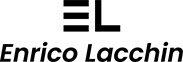
\includegraphics[width=0.3\columnwidth]{img/logo_black}}\lfoot{© Enrico Lacchin | \url{www.enricolacchin.com}}
\cfoot{}
\rfoot{\thepage}

\leftskip 0.0pt

%----------------------------------------------
% INIZIO DOCUMENTO
%----------------------------------------------
\begin{document}

%----------------------------------------------
% TITOLO
%----------------------------------------------
\pagenumbering{gobble}

\small{Enrico Lacchin}

\MidSep
\textbf{\LARGE{Algoritmi e Strutture dati}}

\MidSep
\textit{\Large{Appunti}}
\Sep

\begin{center}
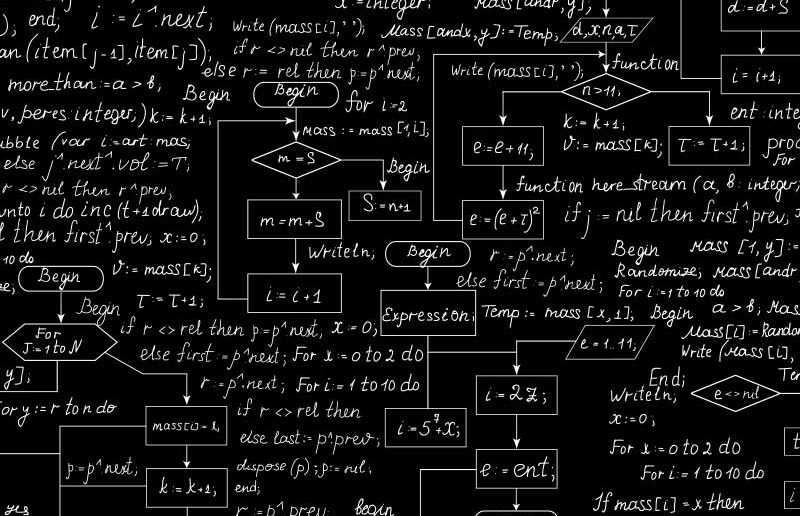
\includegraphics[width=1\columnwidth]{img/algoritmo.jpg}
\end{center}

\vfill
Materia: Algoritmi e strutture dati

Docente: << Nome Docente >>
%----------------------------------------------
% INDICE
%----------------------------------------------

\clearpage
\pagenumbering{roman}
\setcounter{page}{1}
\tableofcontents

%----------------------------------------------
% INIZIO CAPITOLI
%----------------------------------------------
%CAPITOLO 1
\clearpage

\pagenumbering{arabic}
\setcounter{page}{1}

\section{Algoritmo}
Un algoritmo è un procedimento di calcolo teoricamente meccanizzabile. Rappresenta la \textsl{sequenza di passi computazionali che prende in ingresso un dato insieme di valori e produce un insieme di valori in uscita}.\\
Un algoritmo viene usato come strumento per risolvere un ben definito problema computazionale.\\
Un algoritmo può essere:\begin{itemize}
\item \textbf{Corretto}: termina con insieme corretto di valori in uscita per ogni istanza del problema
\item \textbf{Incorretto}: termina o con un insieme non corretto di valori in uscita per alcune istanze del problema oppure non termina.
\end{itemize}
Ogni algoritmo ha una propria \textbf{efficienza} ossia il numero di operazioni richieste per produrre dati in uscita (considerando quelli in entrata) $\rightarrow$ con dimensioni notevoli la differenza di efficienza è marcata.\\
Le \textbf{proprietà} di un'algoritmo sono:
\begin{itemize}
\item Non ambiguità
\item Finitezza
\item Terminazione
\item Effettività
\item Atomicità (operazioni minime)
\end{itemize}

\SmallSep \noindent
Un \textbf{array} è una lista ad accesso diretto (non sequenziale) casuale (dove vogliamo).\\
L'\textbf{istanza} di un problema è l'insieme dato di valori in ingresso.\\
La \textbf{struttura dati} è la modalità di memorizzazione e organizzazione di dati per garantire un miglior accesso e manipolazione. Una struttura dati è la \textsl{heap} la quale organizza array per verificare la proprietà detta priorità (alternativa: albero binario quasi completo).

%CAPITOLO 2
\clearpage
\section{Analisi}
L'analisi va a stimare le risorse richieste in memoria, la banda e il tempo di calcolo.\\
Il \textbf{modello del calcolatore} da usare è:
\begin{itemize}
\item Singolo processore (Single Core)
\item Memoria ad accesso casuale
\item No gerarchie di memoria
\end{itemize}
Le \textbf{assunzioni} sono istruzioni varie con periodo costante.\\
Il \textbf{tempo di esecuzione} è la somma dei tempi di esecuzione (costanti per ipotesi) di ciascuna linea dello pseudocodice moltiplicata per il numero di esecuzione della stessa $\rightarrow$ espresso come dimensione dei valori in ingresso.\\
Tipologie di assunzioni:
\begin{itemize}
\item Ordinamento: lunghezza della sequenza da ordinare $\rightarrow$ divide et impera come metodo di risoluzione efficiente
\begin{itemize}
\item suddivisione del problema in sottoproblemi più semplici
\item risoluzione ricorsiva dei sottoproblemi
\item combinazione delle soluzioni per soluzione del problema
\end{itemize}
\item Operazioni sui grafi: numero di vertici e archi presenti
\end{itemize}

%CAPITOLO 3
\clearpage
\section{Complessità}
\subsection{Classi di complessità}
\begin{equation*}
\begin{array}{lll}
f(n)=O(g(n)) & \text{equivale a} & a \leq b\\
f(n)=\Omega(g(n)) & \text{equivale a} & a \geq b\\
f(n)=\Theta(g(n)) & \text{equivale a} & a = b\\
f(n)=o(g(n)) & \text{equivale a} & a < b\\
f(n)=\omega(g(n)) & \text{equivale a} & a > b\\
\end{array}
\end{equation*}
\textbf{Caso peggiore} (worst case): Si svolgono tutte le iterazioni possibili all'interno dell'algoritmo\\
\textbf{Caso medio} (medium case): \'E a metà tra il caso migliore e il caso peggiore\\
\textbf{Caso migliore} (better case): Si svolgono il minor numero di iterazioni possibili all'interno dell'algoritmo\\
\\
\textcolor{blue}{Esempi}:
\begin{center}
\begin{tabular}{l|ll}
Algoritmo & Tempo di esecuzione nel caso peggiore & Tempo di esecuzione atteso/nel caso medio\\ \hline
Insertion sort & $\Theta(n^2)$ & $\Theta(n^2)$\\
Merge sort & $\Theta(n\cdot log(n))$ &  $\Theta(n\cdot log(n))$\\
Heapsort &  $O(n\cdot log(n))$ & ---\\
Quicksort & $\Theta(n^2)$ & $\Theta(n\cdot log(n))$ (atteso)\\
Counting sort & $\Theta(k+n)$ & $\Theta(k+n)$\\
Radix sort & $\Theta(d(n+k))$ & $\Theta(d(n+k))$\\
Bucket sort & $\Theta(n^2)$ & $\Theta(n)$ (caso medio)
\end{tabular}
\end{center}

%CAPITOLO 4
\clearpage
\section{Grafo}
Un grafo è una configurazione formata da un insieme di punti e linee con unione di coppie di nodi $\rightarrow$ definita relazione qualsiasi tipo.\\
Un grafo può essere:
\begin{itemize}
\item \textbf{Semplice}: coppie di vertici non ordinate (simmetria) e distinte
\begin{itemize}
\item Nodi o Vertici (v): singoli punti $\rightarrow$ senza figli: foglie
\item Archi/Edge (E): linee
\item Grado/Degree: numero di archi che partono dal vertice
\item Memoria: Theta di $(v+E)$
\item Complessità $\begin{array}{l}\text{lista di adiacenza: } \Theta 2(|V|+|E|)\\\text{matrice di adiacenza: }\Theta(|V|^2)\end{array}$
\end{itemize}
\item \textbf{Multigrafo}: stesso arco può comparire più volte
\begin{itemize}
\item Molteplicità dell'arco: numero di volte che si ripete
\item Cappi o Loops: contribuisce due volte al grado
\item Complessità: $\Theta(|V|^2)$
\end{itemize}
\end{itemize}


%CAPITOLO 5
\clearpage
\section{Ricorrenza}
La ricorrenza è un equazione o disequazione per descrivere la funzione in termini del suo valore sugli ingressi con dimensione inferiore.\\
Il tempo di esecuzione viene spesso espresso come ricorrenza\\
Metodi di risoluzione:
\begin{itemize}
\item Sostituzione
\begin{itemize}
\item fare una previsione della soluzione
\item verificare l'ipotesi tramite induzione
\end{itemize}
\item Albero della ricorrenza: si crea un albero ricorsivo (generare buone soluzioni di tentativi)
\item Esperto: basata sul teorema dell'esperto (algoritmi ricorsivi)
\end{itemize}

\subsection{Master Theorem (per gli algoritmi ricorsivi)}
Siano $a \geq 1,\ b> 1,\ T(n)=aT\left({n \over b}\right)+f(n),\ \varphi(n)=n^{log_b(a)+ \dots \ \epsilon > 0}$\\
Se \begin{itemize}
\item[i.] $$\lim_{n \to +\infty}{f(n) \over \varphi(n)}=0 \longrightarrow f(n) \in O(n^{log_b(a)-\epsilon})$$
\item[ii.] $$\lim_{n \to +\infty}{f(n) \over \varphi(n)}=l \in \R \longrightarrow f(n) \in \Theta(n^{log_b(a)})$$
\item[iii.] $$\lim_{n \to +\infty}{f(n) \over \varphi(n)}=+\infty \longrightarrow f(n) \in \Omega\left(n^{log_b(a)+\epsilon}\right) \land af({n\over b}) < cf(n) \ per \ qualche\ c<1$$
\end{itemize}
Allora \begin{itemize}
\item[i.] $T(n) \in \Theta(n^{lob_b(a)}) \rightarrow T(n)\in \Theta(\varphi(n))$
\item[ii.] $T(n) \in \Theta\left(n^{lob_b(a)}\cdot log (n)\right) \rightarrow T(n)\in \Theta(\varphi(n)\cdot log(n))$
\item[iii.]$T(n) \in \Theta(f(n)) \rightarrow T(n)\in \Theta(f(n))$
\end{itemize}

%CAPITOLO 6
\clearpage
\section{Struttura dati}
\textbf{Array}: struttura dati ad accesso libero $\rightarrow$ staticità (bisogna sapere $n$ a priori)\\
\textbf{List/Lista concatenata}: ad accesso sequenziale. L'\textsl{insert} è sempre possibile mentre il \textsl{delete} solo se il contenuto $\geq 1 \rightarrow$ dinamicità.\\
L'inizio viene definito come \textcolor{red}{head} e la fine come \textcolor{red}{tail}.\\
Ci sono due tipologie: \begin{itemize}
\item FIFO (First In First Out): elementi aggiunti da una parte e estratti dall'altra $\rightarrow$ code (queue)
\item LIFO (Last In First Out): elementi aggiunti e tolti dalla stessa parte $\rightarrow$ pile (stack)
\end{itemize}
Un \textbf{record} è la raccorta di dati o numeri $\rightarrow$ \begin{tabular}{l}key: valore da ordinare\\altri valori: dati satelliti \end{tabular}

%CAPITOLO 7
\clearpage
\section{Algoritmi di ordinamento}
\subsection{Bubble Sort}
Ogni coppia di elementi adiacenti comparata se, non in ordine, vengono invertiti.\\
Complessità: $\Theta(n)$ nel caso migliore $\rightarrow$ controlli inutili se gli elementi sono già in ordine.

\subsection{Exhaustive Search}
Va a verificare ogni soluzione teoricamente possibile fino a quella corretta.\\
Risulta essere estremamente lento ma corretto e va sfruttato solo con pochissimi elementi.\\
Complessità: $\Theta(2^n)$

\subsection{Heapsort}
L'algoritmo va a ordinare dall'alto verso il basso.\\
L'\textbf{altezza di un nodo} è la lunghezza degli archi del percorso più semplice verso una foglia. L'\textbf{altezza heap} rappresenta l'altezza della radice.\\
La dimensione del problema varia a seconda del tipo di problema: \begin{itemize}
\item Originario: $n$
\item Sottoalbero con più elementi: $m$
\item Altezza del nodo oggetto del problema originario: $h$
\end{itemize}

\subsection{Mergesort}
L'algoritmo va a suddividere $n$ elementi in sottosequenze di ${n\over 2}$ elementi della stessa dimensione (approccio divide et impera).\\
Non fa ordinamento in loco, fa un ordinamento ricorsivo delle sottosequenze fino a una sottosequenza di lunghezza 1 (ordinata).\\
Utilizza le funzioni
\begin{itemize}
\item Merge: combinazione di due sottosequenze ordinate per produrre intera sequenza ordinata $\rightarrow$ Complessità: $\Theta(n)$
\item Mergesort: ordinamento di una sequenza suddividendola in due, ogni sottosequenza ordinata (con ricorsione) tramite merge
\end{itemize}

%CAPITOLO 8
\clearpage
\section{Ordinamento per confronti}
\paragraph{Teorema}: Qualsiasi algoritmo per confronti ha $\Omega(n\cdot log(n))$ nel caso peggiore

\subsection{Bucket Sort}
\'E un algoritmo molto frequente. Ipotesi di elementi distribuiti uniformemente $\rightarrow \ n$ elementi da ordinare.\\
\textbf{Procedimento}:
\begin{itemize}
\item intervallo $[0,1)$ diviso in $n$ intervalli/contenitori (bucket) di lunghezza uguale
\item ciascun valore dell'array inserito nel bucket a cui appartiene
\item valori all'interno del bucket ordinati
\item concatenazione dei valori contenuti nei bucket con insertion sort
\end{itemize} 

\subsection{Insertion Sort}
L'algoritmo va a considerare un valore alla volta e lo si mette nella posizione corretta tra i valori che lo precedono (approccio incrementale).\\
Fa un ordinamento in loco (sul posto). Valori ordinati dell'array con al più un numero costante di essi all'esterno.\\
\'E invariante cioè per ciascuna iterazione, gli elementi originali rimangono gli stessi, ma in ordine crescente\\
\begin{itemize}
\item Vero prima del ciclo
\item Se vero per prima iterazione, vero per l'iterazione successiva
\item Prova che algoritmo corretto quando il ciclo termina
\end{itemize}
Complessità: $\Theta(n)$ nel caso migliore (better sort)

\subsection{Counting Sort (tre indici)}
Non viene fatto un ordinamento in loco. I numeri da ordinare sono compresi tra 0 e $k$ con $k\ll n$ ($k$ molto minore di $n$).\\
\textbf{Procedimento}:
\begin{itemize}
\item Due array, con con $n$ elementi ($A$) e uno vuoto ($B$) $\rightarrow \ A$ parte da 1 ($A=1,0,0,2,2,1$)
\item Altro array riempito tutto di zeri ($C$) $\rightarrow$ la prima casella parte da $0$
\item Si considerano gli elementi di $A \ \rightarrow$ caselle di $C$ corrispondenti agli elementi di $A$ con numeri in cui compaiono ($C = 2, 2, 2$)
\item Si sommano le celle di $C$ con quelle precedenti ($C=2,2,2\ \rightarrow \ C=2,4,6$)
\item Array $B$ di lunghezza $n$ come $A\ \rightarrow$ la prima casella parte da 1
\item Controllo di $A$ dall'ultima alla prima casella
\item Si confrontano i numeri anche tramite il numero della casella $\rightarrow$ si scala $C$ dopo aver messo il numero di $B$
\end{itemize} 
Diventa disastroso con $n^2$. \'E un algoritmo corretto e stabile (numeri con stesso valore nell’array nello stesso ordine sia in input che in output).\\
Complessità dei cicli for: $\Theta(k), (n), (k), (n) \rightarrow$ totale: $\Theta(k+n)$

%CAPITOLO 9
\clearpage
\section{Algoritmi di vista}
Algoritmi per cubo $n-dimensionale$
\begin{itemize}
\item Ogni vertice con $n$ archi
\item Anche con loops e molteplicità, complessità invariata
\end{itemize}

\subsection{Teorema (Handshake Theorem)}
$$\sum_{v \in V} deg(v) = 2|\xi| \Rightarrow \text{La somma dei gradi è sempre pari}$$
Nota: vero anche perché i loops valgono 2

%CAPITOLO 10
\clearpage
\section{Visita di un grafo}
La visita di un grafo significa esaminare una volta tutti i nodi del grafo.\\
Le difficoltà possono essere due: \begin{itemize}
\item Cicli (marcare nodi visitati)
\item Nodi isolati: la visita termina dopo aver considerato tutte le componenti isolate di un grafo
\end{itemize}

\subsection{In ampiezza (BFS, Bread-First-Search)}
Conta la distanza (numero minimo di archi) dal vertice sorgente agli altri punti (se la distanza è infinita, non ci sono cammini disponibili).\\
Per capire se i vertici sono scoperti o meno si utilizza una classificazione per colori:
\begin{itemize}
\item Bianco (W): inizialmente tutti bianchi
\item Grigio (G): incontrato per la prima volta
\item Nero (B): tutti adiacenti di un nodo grigio visitati $\rightarrow$ un nodo nero ha solo adiacenti grigi
\end{itemize}
Grafo dei predecessori: albero
Complessità: $O(V+E)$, se denso $O(E)$

\subsection{In profondità (DFS, Depth-First-Search)}
\textbf{Procedimento}:
\begin{itemize}
\item Si esplorano i nodi degli archi uscenti
\item Backtrack: nodi degli archi uscenti esplorati, si torna indietro per esplorare quelli del predecessore
\item Tutti i vertici raggiunti da una sorgente iniziale $\rightarrow$ se alcuni vertici sono inesplorati, uno viene scelto come nuova sorgente e riparte la ricerca
\end{itemize}
Grafo dei predecessori: foresta

\subsection{Topological Sort (DAG, Direct Acyclic Graph)}
Viene fatto un ordinamento lineare di tutti i vertici di un grafo orientato senza cicli $\rightarrow$ i vertici si definiscono ordinati se ogni nodo viene prima dei nodi collegati ai suoi archi uscenti.\\
Non vi è um ordinamento notale $\rightarrow$ la soluzione non è necessariamente unica\\
\textbf{Procedimento}:
\begin{itemize}
\item Si considera una situazione
\item Si parte da un punto arbitrario
\item Si segue la direzione degli archi uscenti
\item Finisti gli archi uscenti, si torna al punto considerato
\item Si ripete dal secondo punto, finché non rimangono più punti
\item Metterli in fila, considerandoli al contrario rispetto a come sono stati ordinati (numero più grande)
\item Ordine rispettato
\end{itemize}

%CAPITOLO 11
\clearpage
\section{Altri algoritmi}
\subsection{Algoritmo di Dijkstra}
L'algoritmo presenza un costo per arco = grafi pesanti mediante numeri $\rightarrow$ necessità di archi non negativi (altrimenti Bellman - Ford)\\
Percorso con costo minimo dal vertice sorgente agli altri. Non serve molteplicità degli archi $\rightarrow$ viene eliminato quello dal costo maggiore.\\
\textbf{Procedimento}:
\begin{itemize}
\item Si prende in considerazione un grafo arbitrario
\item Si considera un vertice come sorgente
\item Si prendono singolarmente i costi delle distanze dal vertice sorgente agli altri $\rightarrow$ si considerano anche i punti per cui si deve per forza passare (se dal vertice sorgente $v_2$, bisogna passare per $v_1$, si considera anche $v_1$)
\item Si eliminano i percorsi più costosi, via via che si trovano
\item L'unico che rimane è il percorso meno costoso
\end{itemize}

\subsection{Algoritmo di Euclide}
L'algoritmo trova il MCD tra due numeri, se ricorsivo richiama se stesso.

%CAPITOLO 12
\clearpage
\section{Distanza di edit}
Si parte da una stringa e la si trasforma in un'altra $\rightarrow$ trasformazioni di costo 1 (tranne gratis che non costa nulla)
\begin{center}
\begin{tabular}{llc}
C & Cancellazione & $\downarrow$\\
I & Inserimento & $\rightarrow$\\
S & Sostituzione & $\searrow$\\
G & Riporto gratis & $\searrow$\\
& $ I \leq C \leq S$ & 
\end{tabular}
\end{center}
\textbf{Procedimento}:
\begin{itemize}
\item Si crea una matrice $\rightarrow$ in alto la parola a cui si vuole arrivare, a sinistra la parola da sui si parte
\item Si tiene uno spazio vuoto da un puntino
\item Si procede a costruire la matrice con numeri
\item Si considera il percorso meno costoso
\item Si fanno le varie trasformazioni e si considerano al contrario
\end{itemize}
Complessità: $\Theta(n^2)$

%CAPITOLO 13
\clearpage
\section{Generazione di Bit pseudocasuali}
\begin{center}
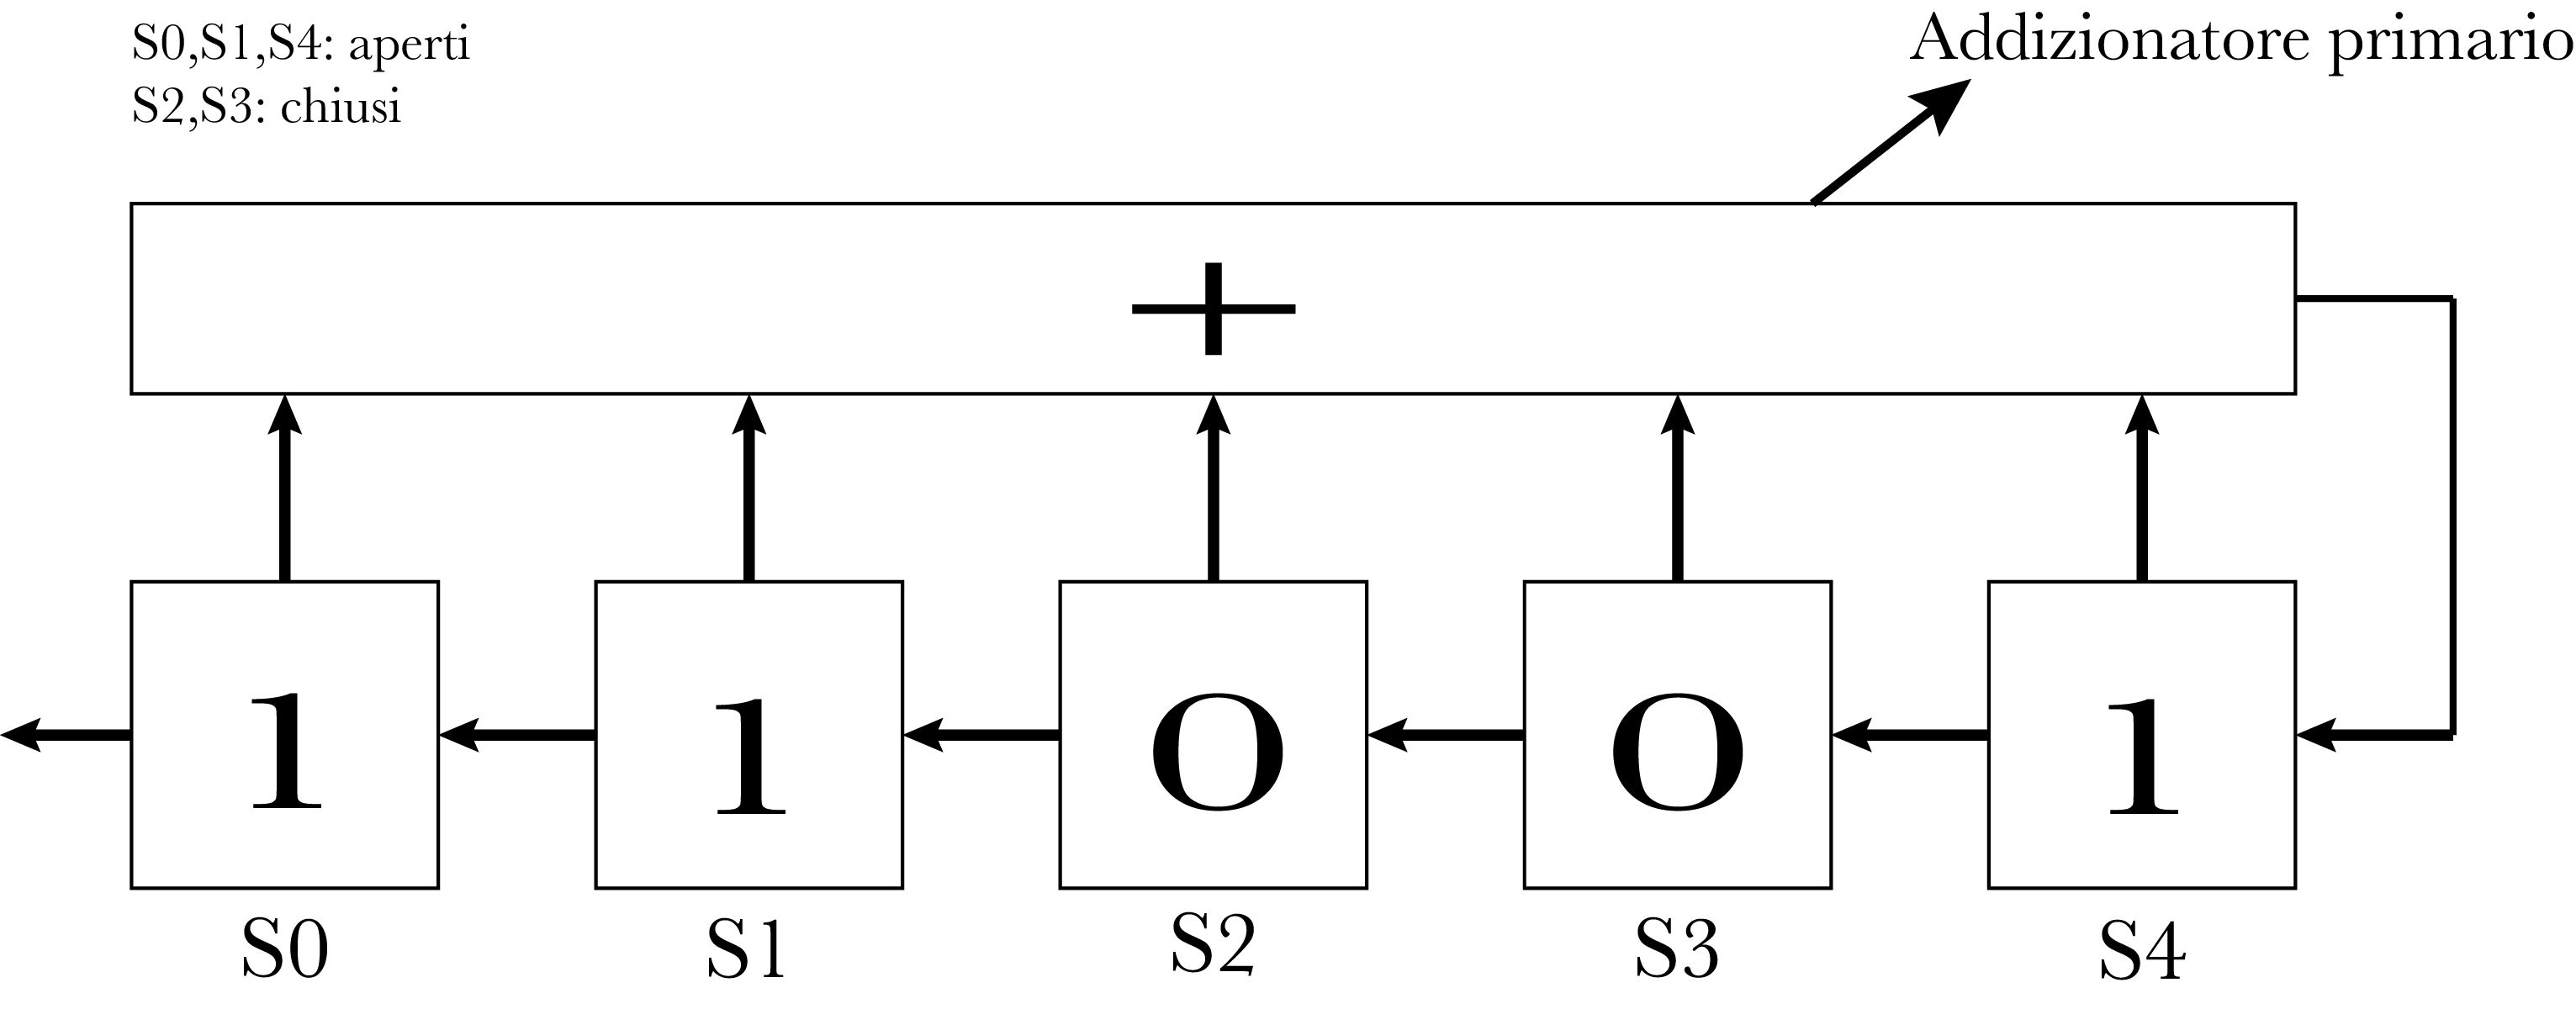
\includegraphics[width=1\columnwidth]{img/bit_pseudocasuali.png}
\end{center}
$$p(x)\hat = a_0 + a_1x + \dots + a_{n-1}x^{n-1} +x^n$$
\begin{center}
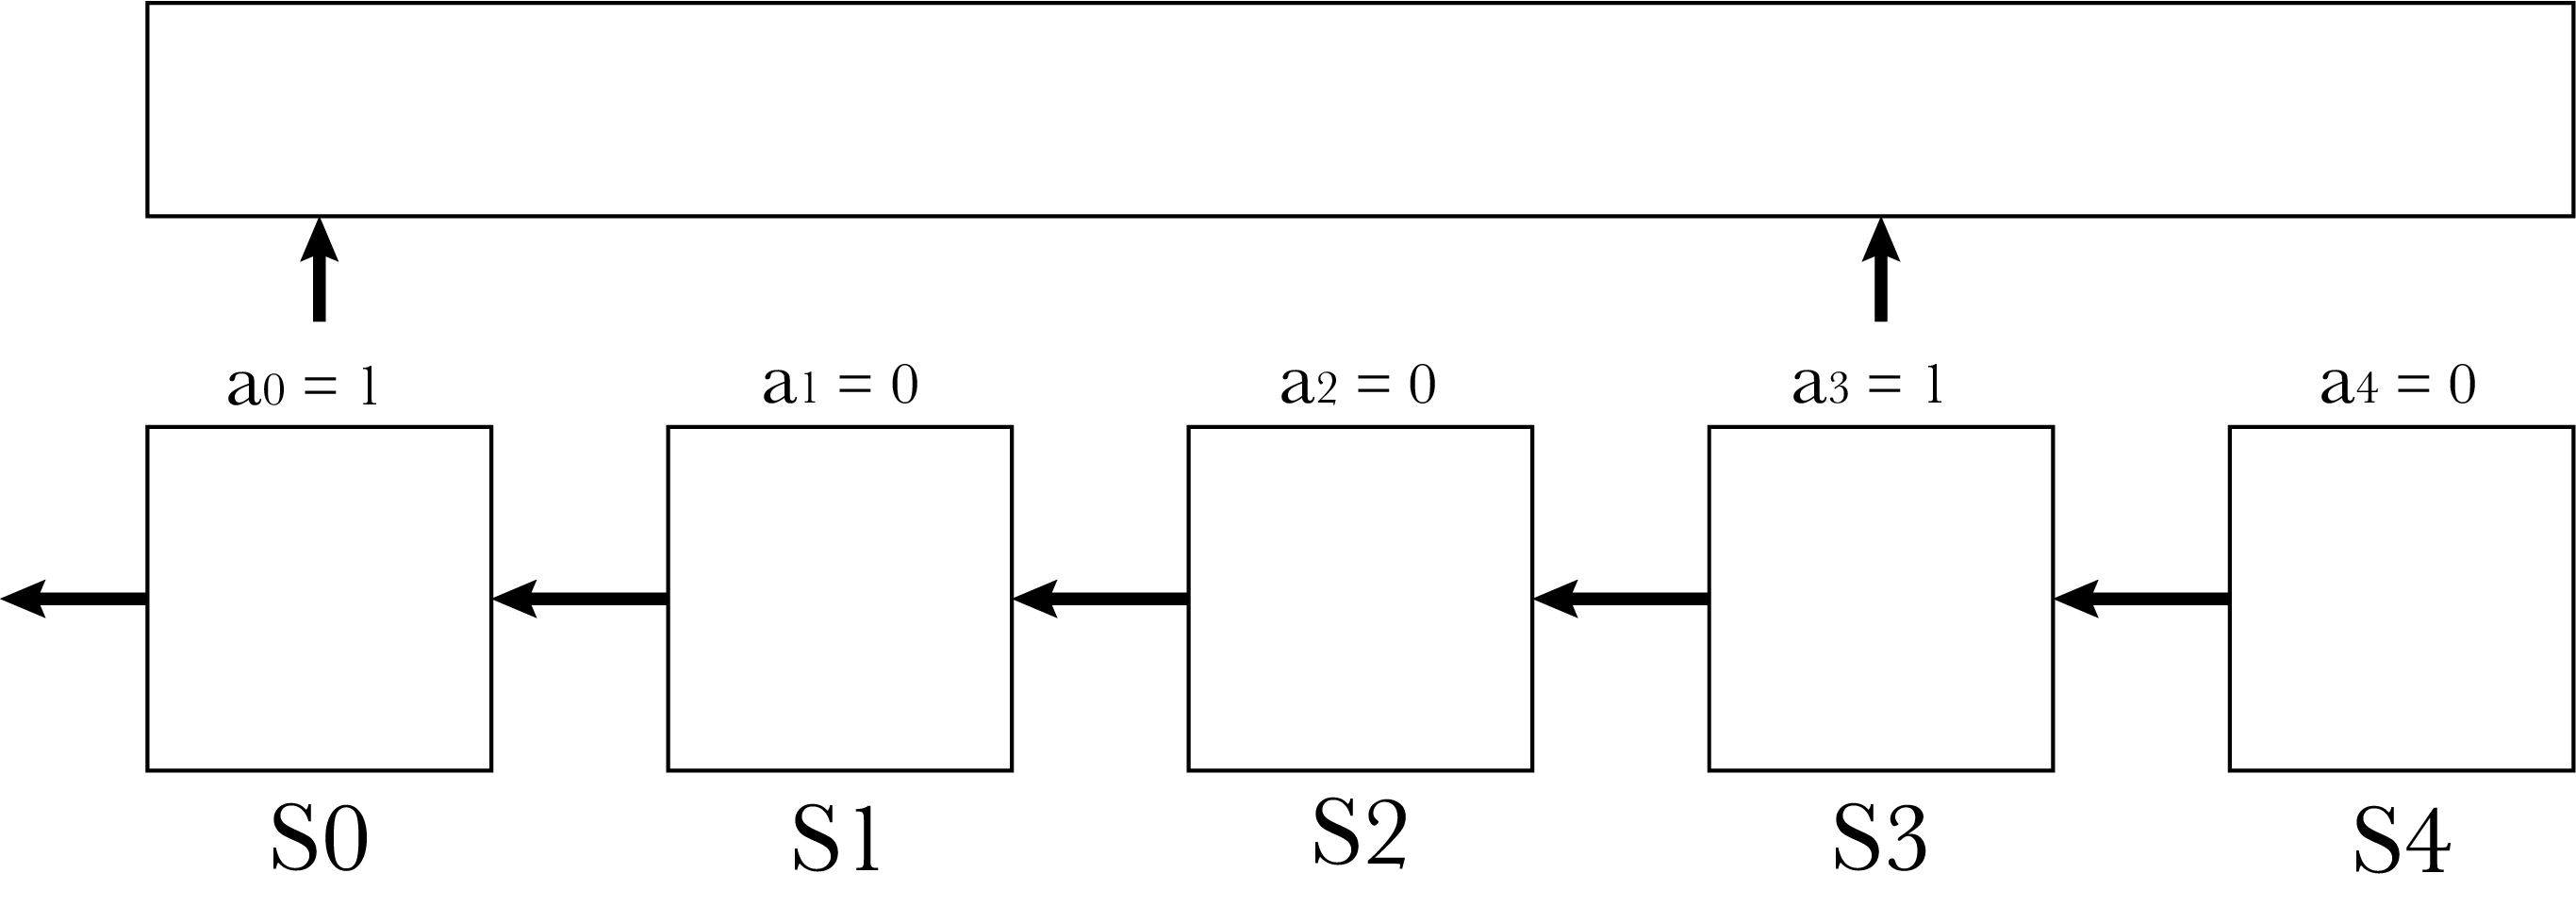
\includegraphics[width=0.7\columnwidth]{img/bit_pseudocasuali_bis.png}
\end{center}
$$p(x)=1+x^3+x^5$$
Registro a scorrimento (verso sinistra) $\rightarrow$ considerati gli spazi dove c'è 1\\
\textbf{Seme}: Combinazione casuale di 0 e 1 $\rightarrow$ proibito: $0\dots0$ dato che la somma fa sempre 0\\
\textbf{Produzione ciclica di periodo massimo}: $2^n -1 \ n-ple$ binarie con accesso "casuale" ($0$ uscenti uguali e $1$ entranti)
\begin{itemize}
\item $n$: lunghezza del registro
\item $1$: seme proibito\\
$\rightarrow$ funzione di autocorrelazione: bilanciamento del numero di $n-ple$ che finiscono con $00,01,10,11$ $[(n-2)-ple$ binarie per ciascuno$]$
\end{itemize}
Shift register circa potenziatore di casualità (data del seme) $\rightarrow$ input determinato

\subsection{Heapify}
Il suo scopo è quello di riorganizzare heap per mantenere la proprietà della priorità.\\
\textbf{Albero}: grafo non diretto, connesso e aciclico $\rightarrow$ grafo di un nodo: numero di sottoalberi del nodo uguale al numero di figli del nodo\\
\textbf{Altezza o profondità dell'albero}: distanza radice - foglia\\
\textbf{Percorrenza}: dalla radice verso le foglie (dall'alto verso il basso)\\
$|E|=|V|-1$\\
Complessità: $\Theta(n)$

\subsection{Quicksort}
\begin{center}
\includegraphics[width=1\columnwidth]{img/quicksort.png}
\end{center}
\textbf{i} (wall): non è detto che si sposti\\
\textbf{j} (current element): si sposta di una posizione alla volta\\
\textbf{Pivot}: elemento considerato\\
Viene utilizzato l'approccio del divide et impera.\\
\textbf{Partition} (prima parte di quicksort)
\begin{itemize}
\item Si fissa il pivot\\
\item Si inizializza il muro\\
\end{itemize}
Quicksort $\rightarrow$ si mettono i valori come nell'immagine\\
Randompartition $\rightarrow$ il primo dei più grandi e pivot scambiati

%CAPITOLO 14
\clearpage
\section{Problemi famosi}
\subsection{Hamilton}
\begin{center}
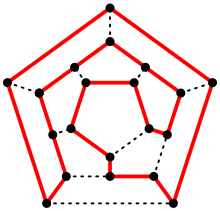
\includegraphics[width=0.4\columnwidth]{img/hamilton.png}
\end{center}
\textbf{Icosaedro}: Qualsiasi poliedro a 20 facce\\
Nel solido platonico le facce sono separate da spigoli (edge).\\
Si può, in due dimensioni, toccare tutti i vertici una sola volta (closed path)? La risposta è NO, non esiste un algoritmo che risolva il problema ($P \not = NP$)

\subsection{Eulero}
\begin{center}
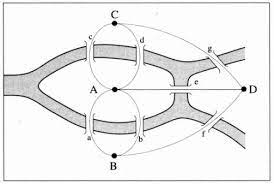
\includegraphics[width=0.4\columnwidth]{img/eulero.jpeg}
\end{center}
K\"onigsberg è una città collegata da 7 ponti.\\
\textbf{Problema}: Fare una passeggiata passando per ciascun ponte una sola volta\\
\textbf{Soluzione}: Non è possibile, dato che il numero dei gradi di ciascuna zona è dispari.\\

\subsection{Sacco o Knapsack Problem}
Il problema di Knapsack è un problema di ottimizzazione.\\
Il ladro che ruba deve prendere in considerazione:
\begin{itemize}
\item $H$: altezza del sacco/zaino
\item $h$: altezza dell'oggetto che vuole rubare
\item $v$:  valore dell'oggetto che vuole rubare
\end{itemize}
\textbf{Greedy}: il ladro ruba fino a quando ha spazio, anche se potrebbe prendere oggetti senza valore.\\
Complessità: $\Theta(n^2)$ nel caso peggiore\\
\textbf{Greedy con preordinamento}: Il ladro mette all'inizio gli oggetti più preziosi e quelli vengono rubati.\\
Complessità: $\Theta(n^2)$ nel caso peggiore

%CAPITOLO 15
\clearpage
\section{Altro}
\subsection{LCS}
$$X=<x_1, \dots, x_m>\ \ e \ \ Y=<y_1, \dots, y_n>$$
\begin{enumerate}
\item Caratterizzazione: $2^m$ sottosequenze di $X$ $\rightarrow$ tempo esponenziale (inutilizzabile con lunghe sequenze)
\item Soluzione ricorsiva
\item Calcolo della lunghezza con il metodo bottom-up\\
$\Theta(m\cdot n)$ sottoproblemi
\end{enumerate}

\subsection{Problemi}
\begin{itemize}
\item \textbf{P}: risolvibili in un tempo polinomiale $\rightarrow$ nel caso peggiore $O(n^k)$ con $k$ costante
\item \textbf{NP}: non risolvibili in un tempo polinomiale (e.g. problema di Hamilton) $\rightarrow$ C / completo: particolarmente difficili da risolvere. Se si può risolvere un elemento di NPC in tempo polinomiale, lo si può fare con qualsiasi elemento (ancora non trovato)\\
\end{itemize}
Si ipotizza $P \not = NP$ oppure $P\subset NP$, ma non dimostrato


%----------------------------------------------
% FINE DOCUMENTO
%----------------------------------------------
\end{document}